\chapter{Mathematical Methods}\label{ch:math}

\section{Diffusion maps} \label{sec:dmaps}

Diffusion maps is an unsupervised, nonlinear data mining algorithm. 
%
Given points which lie on a low-dimensional manifold in a high-dimensional space, diffusion maps uncovers a parameterization of the data which captures the notion of locality with respect to the manifold. 
%
%Diffusion maps is the generalization of Laplacian Eigenmaps \cite{Belkin2003}, and is the culmination of advances in nonlinear data mining over the past twenty years \citep{Donoho2003,roweis2000nonlinear,tenenbaum2000global}.

Given $\ndata$ data points $\data(1), \dots, \data(\ndata)$ (typically vectors in a high-dimensional vector space) which lie on a lower-dimensional manifold $\manifold$, the goal is to find a coordinate transformation $f(\data)$ that preserves local geometry: points that are ``close" in the original space should also be ``close" in the coordinates $f$.
%
%From pairwise distances, we want to extract a {\em global} parametrization of the data that represents the slow variables.
%
%We will use diffusion maps \cite{Coifman2006, coifman2005geometric}, a kernel-based manifold learning technique, to extract a global parametrization using the local distances.
%
We first construct the kernel matrix $\mathbf{W} \in \mathbb{R}^{\ndata \times \ndata}$, where
\begin{equation} \label{eq:dmaps_kernel}
W_{ij} = \exp \left( -\frac{\|\data(i) - \data(j) \|^2}{\dmeps^2} \right).
\end{equation}
Here, $\| \cdot \|$ denotes the appropriate norm, and $\dmeps$ is the kernel scale
and denotes a characteristic distance within the data set.
%
Note that $\dmeps$ induces a notion of locality: if $\|\data(i) - \data(j) \| \gg \dmeps$, then $W_{ij}$ is negligible.
%
Therefore, we only need our metric to be informative within a ball of radius $\dmeps$.
%
Points less than $\dmeps$ apart are thus considered ``close'' and points farther than $\dmeps$ apart are considered ``far away''.
%
$\dmeps$ can be chosen using several techniques (see, for example \citep{coifman2008graph, rohrdanz2011determination}).
%
We often use the median of the pairwise distances as $\dmeps$, as it empirically often yields good results (since each data point is connected to approximately half of the other data points), and does not require any manual input. 

%We note that the eigenvectors $\phi_0, \dots, \phi_{\ndata-1}$ solve the following optimization problem \citep{Belkin2003}
We then consider solving the following optimization problem \citep{Belkin2003}
\begin{equation} \label{eq:dmaps_opt_problem}
\argmin_{f} \sum_{ij} W_{ij} (f(\data(i)) - f(\data(j)))^2.
\end{equation}
%
Because of our definition of the matrix $\mathbf{W}$, solving this optimization problem will preserve local geometry, such that $f(\data(i))$ and $f(\data(j))$ will be similar if $\data(i)$ and $\data(j)$ are close. 
%
To solve \eqref{eq:dmaps_opt_problem}, we construct the diagonal matrix $\mathbf{D} \in \mathbb{R}^{\ndata \times \ndata}$, with
\begin{equation}
D_{ii} = \sum_{j=1}^\ndata W_{ij}.
\end{equation}
%
We compute the eigenvalues $\lambda_0, \dots, \lambda_{\ndata-1}$ and eigenvectors $\phi_0, \dots, \phi_{\ndata-1}$ of the matrix $\mathbf{A} = \mathbf{D}^{-1}\mathbf{W}$, and order them such that $1 = \lambda_0 \ge |\lambda_1| \ge \dots \ge |\lambda_{\ndata-1}|$.
%
The eigenvectors are then solutions to \eqref{eq:dmaps_opt_problem}, such that each each eigenvector is a solution which is orthogonal to the previous eigenvector solutions. 
%
Because the matrix $\mathbf{A}$ is row-stochastic, the first eigenvector will always be the trivial eigenvector $\phi_0 = \begin{bmatrix} 1 & 1 & \cdots & 1 \end{bmatrix}^T$ (which corresponds to a trivial solution to \eqref{eq:dmaps_opt_problem}).
%
The next few eigenvectors provide embedding coordinates for the data, so that $\phi_j(i)$, the $i^{th}$ entry of $\phi_j$, provides the $j^{th}$ embedding coordinate for $\data(i)$ (modulo higher harmonics which characterize
the same direction in the data; see \cite{ferguson2010systematic} and \chap~\ref{ch:harmonics}).
%
The mapping
\begin{equation} \label{eq:dmaps_embed_full}
\data(i) \mapsto 
\begin{pmatrix}
\lambda_1^t \phi_1(i) \\
\lambda_2^t \phi_2(i) \\
\vdots \\
\lambda_{\ndata-1}^t  \phi_{\ndata-1}(i)
\end{pmatrix}
\end{equation}
is the diffusion maps embedding for the data, where $t > 0$ is a parameter.
%
We typically take $t=0$ in our analysis, which corresponds to the Laplacian Eigenmaps embedding.  
%
We then define the diffusion distance $D_t (\data(i), \data(j))$ as 
\begin{equation}
D_t^2 (\data(i), \data(j)) = \sum_{k=1}^{\ndata-1} \lambda_k^{2t} \left( \phi_k(i)- \phi_k(j) \right)^2.
\end{equation}
%
The diffusion maps embedding therefore projects the data into a space where the Euclidean distance is equivalent to the diffusion distance. 
%
If the eigenvalues exhibit a spectral gap, where $|\lambda_1| \ge |\lambda_2| \ge \dots \ge |\lambda_\lowdim | \gg |\lambda_{\lowdim+1} | \ge \dots \ge |\lambda_{\ndata-1}|$, then one can embed the data in the first $\lowdim$ eigenvectors, 
\begin{equation} \label{eq:dmaps_embed_reduced}
\data(i) \mapsto 
\begin{pmatrix}
\lambda_1^t \phi_1(i) \\
\lambda_2^t \phi_2(i) \\
\vdots \\
\lambda_{\lowdim}^t  \phi_{\lowdim}(i)
\end{pmatrix}
\end{equation}
%
while still approximately retaining the diffusion distance. 


%This is analogous to how the eigenfunctions $\cos x$ and $\cos 2x$ of the usual Laplacian in one spatial dimension and with no flux boundary conditions are one-to-one with the values of $x$ for $0 \le x \le 1$;
%one must check for correlations between the eigenvectors before selecting those that describe the underlying manifold geometry.




Ignoring the higher harmonics, each retained eigenvector then describes an intrinsic variable for the data set of interest.
%
We note that the eigenvectors can be determined up to a scaling factor.
%
For some applications, the magnitude and/or sign of the eigenvectors are important. 
%
For the work presented in \chap~\ref{ch:merging}, we must normalize the eigenvectors from different data sets so that the resulting embeddings are consistent.
%
We first scale the eigenvectors so that $\|\phi_i\| = \ndata$, where $\ndata$ is the number of data points,
to make the embedding coordinates invariant to the size of the data set.
%twice as many samples as another data set, but with the same underlying geometry, should have twice the norm.
%
Still, the computed embedding eigenvectors, even for two identical data sets, may differ by a sign.
%
Reconciling the signs for the embeddings of different data sets can be rationally done in several ways and is somewhat problem-specific.
%
For example, if the mean of the embedding is sufficiently far from 0, we can require $\langle \phi_i \rangle > 0$;
alternatively, if there is a common region sampled by both data sets, the sign of each eigenvector can be chosen to optimize the consistency of the embeddings of the common region data.
%
%We will return to the issue of embedding consistency for different data sets in our concluding discussion; for the moment, we will assume that our different sets sample the same region of data space in a representative enough way such that the correspondence between the sequences of retained eigenvectors for different embeddings is obvious.
%
Similarly, for the examples in \chap~\ref{ch:drosophila}, the sign of the eigenvector is important, and are determined after analysis using {\em a priori} knowledge of the system. 




\subsection{Family of operators} \label{sec:diff_limit}

In the limit $\dmeps \rightarrow 0$ and $\ndata \rightarrow \infty$, the matrix $\mathbf{I} - \mathbf{A}$ converges to the continuous backward Fokker-Planck operator \cite{nadler2006diffusion}
\begin{equation}
	\mathcal{L} = \Delta - 2 \nabla U \cdot \nabla.
	\label{eq:limiting_operator}
\end{equation}
where the data $\data_1, \dots , \data_\ndata$ are sampled from $\manifold$ with density proportional to $e^{-U}$. 
%
However, we can construct a family of diffusion operators 
\begin{equation} \label{eq:kernel2}
\mathbf{A}^{(\alpha)} = {\mathbf{D}^{(\alpha)}}^{-1} \mathbf{W}^{(\alpha)}
\end{equation}
where $\mathbf{W}^{(\alpha)} = \mathbf{D}^{-\alpha} \mathbf{W} \mathbf{D}^{-\alpha}$ 
and $\mathbf{D}^{(\alpha)}$ is a diagonal matrix with $\mathbf{D}^{(\alpha)}_{ii} = \sum_{j=1}^\ndata \mathbf{W}^{(\alpha)}$.
%
We then have \cite{coifman2005geometric}
\begin{equation}
\begin{aligned}
\mathbf{A}^{(0)} & \rightarrow \Delta - 2 \nabla U \cdot \nabla \\
\mathbf{A}^{(1/2)} & \rightarrow \Delta - \nabla U \cdot \nabla \\
\mathbf{A}^{(1)} & \rightarrow \Delta  
\end{aligned}
\end{equation}
%
Therefore, choosing different values of $\alpha$ results in different kernel normalizations which can remove sampling density effects along the manifold. 


\section{The Mahalanobis distance}
\label{subsec:mahalanobis}

The essential component of manifold learning algorithms (such as diffusion maps) is having an informative distance metric between data points, as one of the key assumptions is that points which are close on the manifold have a small distance. 
%
However, often the Euclidean distance is not informative, and we require a more sophisitcated metric. 
%
Here, we will discuss the Mahalanobis distance \cite{mahalanobis1936generalized}. 
%
This distance has some nice propoerties which will allow us to analyze multiscale stocastic systems in \chap~\ref{ch:multiscale} and data from chemical simulations in \chap~\ref{ch:merging}. 

Let $\mathbf{C}(t)$ be the covariance matrix associated with the measured sample $\data(t)$ (the specifics will be discussed in subsequent chapters). 
%
We define a Riemannian metric between a pair of samples using the associated covariance matrices as
\begin{equation}
	d^2(\data(i), \data(j)) = 2 (\data(i) - \data(j))^T(\widehat{\mathbf{C}}(i) + \widehat{\mathbf{C}}(j))^{\dagger}(\data(i) - \data(j));
	\label{eq:mahalanobis1}
\end{equation}
this is the Mahalanobis distance (and $^{\dagger}$ denotes a pseudoinverse, as discussed below).
%
The covariance matrices convey the local variability of the measurements and are utilized to explore and learn the tangent planes of the observable manifold.
%
This information is then utilized in \eqref{eq:mahalanobis1} to compare a pair of points according to the directions of their respective tangent planes.
%
The Mahalanobis distance is invariant under affine transformations.
%
Thus, by assuming that the observation function $\measfn$ is bi-Lipschitz and smooth, and by using local linearization of the function, i.e., $\data(t) = \mathbf{J}(t) \mathbf{x}(t) + \boldsymbol{\epsilon}(t)$ where $\mathbf{J}(t)$ is the Jacobian of $\measfn(\mathbf{x}(t))$ and $\boldsymbol{\epsilon}(t)$ is the residual consisting of higher-order terms, it was shown by Singer and Coifman \cite{singer2008non} that $\mathbf{C}(t) = \mathbf{J}(t)\mathbf{J}^T(t)$ and that the Mahalanobis distance approximates the Euclidean distance between the corresponding samples of the underlying process to second order, i.e.,
\begin{equation}
	\| \mathbf{x}(i) - \mathbf{x}(j) \|^2 = d^2(\data(i), \data(j)) + \mathcal{O}(\| \data(i) - \data(j)\|^4).
\end{equation}
%
This result implies that the Mahalanobis distance is invariant to the measurement function $\measfn$, and hence,
it yields the same distances between samples obtained under different observation functions or even partial observations.
%
We would like to note that, in general, $\measfn$ being bi-Lipschitz implies that $\measfn$ is invertible (on the $d$-dimensional
manifold $\manifold$).
%
However, in practice, determining whether $\measfn$ contains sufficient information and is ``rich enough'' to completely determine the underlying process is a non-trivial task.
%
In this work, we exploit the fact that $\mathbf{C}(t) = \mathbf{J}(t)\mathbf{J}^T(t)$, which implies that $\mathbf{C}(t)$ is an $\highdim \times \highdim$ positive semidefinite matrix of rank $d$, to empirically infer the dimension $\lowdim$.
%
According to the spectrum of the local covariance matrices and their corresponding spectral gaps, we approximate the rank of the matrices.
%
Consistent rank estimates among these local covariance matrices are taken to imply that the measurements are ``rich enough", and hence, may be good indicators for the dimension $\lowdim$.
%
Since the dimension $\lowdim$ of the underlying process is typically considerably smaller than the dimension of the measured process $\highdim$,
the covariance matrix is singular and non-invertible;
%
thus, we use the pseudo-inverse in \eqref{eq:mahalanobis1}.

In practice, the covariance matrix can be estimated from a short trajectory of samples in time around the sample $\data(t)$ by
\begin{equation} \label{eq:cov1}
	\widehat{\mathbf{C}}(t) = \sum \limits _{\tau = t-L}^{t+L} (\data(\tau) - \widehat{\boldsymbol{\mu}}(t))(\data(\tau) - \widehat{\boldsymbol{\mu}}(t))^T,
\end{equation}
where $\widehat{\boldsymbol{\mu}}(t)$ is the empirical mean of the short trajectory of samples.
%
Alternatively, we can estimate the local covariance by using small bursts of simulation 
\begin{multline} \label{eq:cov2}
\hat{C}_{ij}(\data(t), \delta t)
= \\
\frac{1}{ \delta t} \left( \mathbb{E} \left[ y_i (t+\delta t) y_j (t+ \delta t) \mid \data(t) \right]
- \mathbb{E} \left[ y_i (t+\delta t) \mid \data(t) \right] \mathbb{E} \left[ y_j (t+\delta t) \mid \data(t) \right] \right) ,
\end{multline}
%
where $\delta t > 0$ is the length of the simulation burst.
%
The Mahalanobis distance can also reduce the effects of fast variables, as will be discussed in \chap~\ref{ch:multiscale}.

%\begin{table}[tb]
%\caption{Nonlinear Intrinsic Variables Construction Algorithm}
%\hrule
%\begin{enumerate}
%
%\item
%Obtain a sequence of high-dimensional observation samples $\data(t)$.
%
%\item
%Compute the empirical covariance matrix $\widehat{\mathbf{C}}(t)$ of each sample $\data(t)$ {\em in a short window in time} according to \eqref{eq:cov1} or \eqref{eq:cov2}.
%
%\item
%Using the samples and their associated covariance matrices, compute the Mahalanobis distance between the observations \eqref{eq:mahalanobis1} .
%
%\item
%Build the pairwise affinity matrix $\mathbf{W}$ and the corresponding normalized kernel $\mathbf{W}^{(\alpha)}$ in \eqref{eq:kernel2}.
%
%\item
%Apply eigenvalue decomposition to the normalized kernel and view the values of its principal eigenvectors (modulo the possibility of
% ``higher harmonics", see text) as the Nonlinear Intrinsic Variables (NIV) of the given observations.
%
%\end{enumerate}
%\hrule
%\label{algo}
%\end{table}


\section{Angular synchronization } \label{sec:ang_synch}

The Mahalanobis distance is useful for analyzing data which have been obscured by large noise and/or a measurement function. 
%
Another source of variability that one would often like to factor out is due to symmetries, when data (such as images) are collected in many different orientations. 
%
These orientational differences are an artifact of the experimental or imaging setup and must be factored out for informative analysis.
%
We will discuss two algorithms for registering images with respect to rotational symmetries. 
%
Angular synchronization \cite{singer2011angular} is an algorithm for registering a data set given pairwise alignment information. 
%
Vector diffusion maps \cite{singer2012vector} then combines angular synchronization and diffusion maps to both register and uncover structure in data in a single computation. 
%
We demonstrate these two algorithms for registration and temporal ordering using a synthetic data set.
%
The relatively simple dynamics of this data set allows us to easily visualize and illustrate the main features of the different algorithms.
%
Motivated by the geometry of our {\em Drosophila} embryo images in \chap~\ref{ch:drosophila}, we construct a sequence of concentration profiles defined on a ring, and rotate each ring randomly around its center; an example is shown in \fig~\ref{fig:1d_demo}A.
%
Rotation of the ring corresponds to shifting (with periodic boundary conditions) the one-dimensional concentration profile shown at the bottom of \fig~\ref{fig:1d_demo}A (the symmetry group is $SO(2)$, the group of all two-dimensional proper rotations).
%
Each concentration profile is a noisy Gaussian (shown in \fig~\ref{fig:1d_demo}B), and the Gaussians increase in intensity as a function of ``time".
%
We discretize the profiles into $100$ points, so our numerical data will be $100$-dimensional vectors (the corresponding symmetry group for the discretized profiles is $\mathbb{Z}_{100}$, the group of integers modulo $100$).
%
\fig~\ref{fig:1d_demo}C shows the entire data set; the concentration profiles have been stacked in an array, so that each row corresponds to a single profile.
%
Because the profiles are unregistered and unordered, the underlying dynamics (a Gaussian whose amplitude grows in time) are not readily apparent.

\begin{figure}
\centering
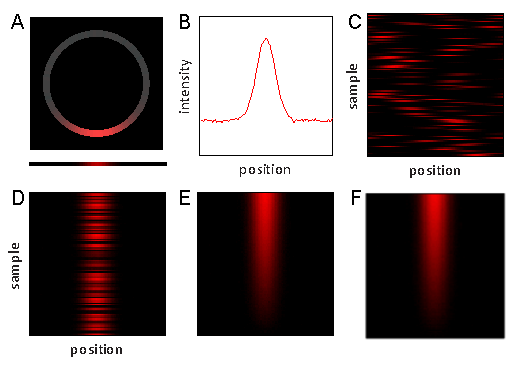
\includegraphics[width=0.8\textwidth]{ch-drosophila/figures/figS2}
\caption[Synthetic data set used to illustrate registration and ordering algorithms]{Synthetic data set used to illustrate the data processing algorithms. (A) One-dimensional concentration profile on a ring (top), and the corresponding profile on a line (bottom). (B) Intensity corresponding to the profile in A. (C) An ensemble of concentration profiles, each of the form described in A. Each row in the array corresponds to a single profile. {(D)} The profiles in {C}, now registered using angular synchronization. {(E)} The profiles in {D}, now temporally ordered using diffusion maps.  {(F)} The profiles in {C}, registered and temporally ordered in a single step using vector diffusion maps.}
\label{fig:1d_demo}
%\customlabel{subfig:1d_example}{\ref{fig:1d_demo}{\it A}}
%\customlabel{subfig:1d_intensity}{\ref{fig:1d_demo}{\it B}}
%\customlabel{subfig:1d_unaligned_unordered}{\ref{fig:1d_demo}{\it C}}
%\customlabel{subfig:1d_aligned_unordered}{\ref{fig:1d_demo}{\it D}}
%\customlabel{subfig:1d_aligned_ordered}{\ref{fig:1d_demo}{\it E}}
%\customlabel{subfig:1d_aligned_ordered_vdm}{\ref{fig:1d_demo}{\it F}}
\end{figure}

The angular synchronization algorithm aligns pairs of data points with respect to a given symmetry group from pairs of alignment measurements \citep{singer2011angular}. 
%
Let $ \data_1, \dots, \data_\ndata$ denote the signals that we wish to align with respect to rotations;
each signal is a function defined on the unit circle (on the plane).
%
First assume that each signal $\data_i$ is a {\it noisy} rotated copy of the underlying signal $\data_{true}$
(which we are {\it not} given), such that
\begin{equation}
\data_i = f(\data_{true}, \theta_i) + \mathbf{\xi}_i
\end{equation}
where the function $f(\data_{true}, \theta_i)$ rotates the signal $x_{true}$ by $\theta_i$ degrees, and $\mathbf{\xi}_i$ is a (typically Gaussian) noise term.
%
Our goal is to recover $\theta_1, \dots, \theta_\ndata$.
%
Up to noise,
\begin{equation} \label{eq:pairwise_rot}
\data_i \approx f(\data_j, \theta_i - \theta_j) ;
\end{equation}
note that \eqref{eq:pairwise_rot} does not require knowledge of $x_{true}$.
%
We can obtain an {\it estimate} of $\theta_i - \theta_j$ by computing the rotation that optimally aligns $\data_j$ to $\data_i$,
i.e., %$\theta_{ij} \approx \theta_i - \theta_j$, where
%
\begin{equation} \label{eq:opt_angle}
\theta_i - \theta_j \approx \theta_{ij} = \argmin_{\theta} \|\data_i - f(\data_j, \theta)\|^2.
\end{equation}
%
Practically, the signals are discretized in a $\highdim$-long vector (the local intensity at $n$ equidistant points around the circle);
rotating the function by an angle $\theta$ then corresponds to cyclically shifting the elements of $\data_i$
by $\frac{\theta_i}{2 \pi} \highdim$ (rounded to the nearest integer to obtain a valid shift).
%
For the one-dimensional discretized profiles shown in \fig~\ref{fig:1d_demo}, we exhaustively search over all $\highdim=100$ possible shifts of the signals to obtain the optimal angles in \eqref{eq:opt_angle}.
%
Alternatively, for continuous signals, an optimization algorithm
can be used \citep{ahuja2007template}.

Rather than work with the angles $\theta_{ij}$ directly, it is more convenient to consider the rotation matrices,
\begin{equation} \label{eq:R_theta}
R(\theta_{ij}) = \begin{bmatrix}
\cos(\theta_{ij}) & -\sin(\theta_{ij}) \\
\sin(\theta_{ij}) & \cos(\theta_{ij})
\end{bmatrix},
\end{equation}
which we can think of as operating on the points of the unit circle (on the plane) on which our signal is defined.
%
Successive rotations correspond to multiplication of the corresponding rotation matrices: $R(\alpha_1 + \alpha_2) = R(\alpha_1) R(\alpha_2)$.
%
Due to the orthogonality of rotation matrices, $R(-\alpha) = R(\alpha)^T$.

Let $d$ denote the dimension of the rotation matrices we are considering (for planar rotations, $R(\theta_{ij}) \in \mathbb{R}^{2 \times 2}$ and $d=2$).
%
We construct the matrix $H \in \mathbb{R}^{\ndata d \times \ndata d}$, where $H$ is an $m \times m$ matrix of $d \times d$ blocks, with the $i,j^{th}$ block of $H$, $H_{ij}$, defined as
\begin{equation} \label{eq:H_to_R}
H_{ij} = R(\theta_{ij}).
\end{equation}
%
%
Under our assumption that $\theta_{ij} \approx \theta_i - \theta_j$, $H_{ij} \approx R(\theta_i) R(\theta_j)^T$
%\begin{equation}
%H_{ij} = R(\theta_{ij}) \approx R(\theta_i - \theta_j) = R(\theta_i) R(-\theta_j) = R(\theta_i) R(\theta_j)^T,
%\end{equation}
 and
\begin{equation} \label{eq:H_low_rank}
	H \approx
	\begin{bmatrix}
	R(\theta_1) \\
	R(\theta_2) \\
	\vdots \\
	R(\theta_\ndata)
	\end{bmatrix}
	\begin{bmatrix}
	R(\theta_1)^T R(\theta_2)^T \dots R(\theta_\ndata)^T
	\end{bmatrix}.
\end{equation}
%
It follows directly from \eqref{eq:H_low_rank} that the top block eigenvector of $H$ contains our best estimates of $R(\theta_1), R(\theta_2), \dots, R(\theta_m)$.
%
Let $\phi_0, \phi_1, \dots, \phi_{\ndata d-1}$ denote the eigenvectors of $H$ ordered so that $|\lambda_0| \ge |\lambda_1| \ge \dots \ge |\lambda_{\ndata d -1}|$, where $\lambda_i$ is the eigenvalue corresponding to $\phi_i$.
%
Then,
\begin{equation} \label{eq:R_hat}
\hat{R} =
\begin{bmatrix}
\hat{R}_1 \\
\hat{R}_2 \\
\vdots \\
\hat{R}_\ndata
\end{bmatrix} =
\begin{bmatrix}
| & | & & | \\
\phi_0 & \phi_1 & \dots & \phi_{d-1} \\
| & | & & |
\end{bmatrix},
\end{equation}
where $\hat{R}_i \in \mathbb{R}^{d \times d}$ is (nearly) the estimate for $R(\theta_i)$.
%
To obtain our estimate of $R(\theta_i$), denoted $R_{i, est}$, we project $\hat{R}_i$ onto the closest orthogonal matrix,
\begin{equation} \label{eq:R_est}
R_{i, est} = U_i V_i^T,
\end{equation}
where $U_i$ and $V_i$ are the left and right singular vectors, respectively, of $\hat{R}_i$.
%
We adjust the sign of $\phi_1$ so that $det(R_{i, est}) = +1$, ensuring proper rotations 
(note that systematically incorporating improper rotations is also possible \citep{goemans1995improved, bandeira2013cheeger}).
%
We estimate $\theta_{i}$ by inverting \eqref{eq:R_theta}, and register the signals by rotating signal $i$ by $-\theta_i$.
%
We note that, in our actual computations, the pairwise rotations $\theta_{ij}$ are computed in a discrete setting, then the overall
synchronization is performed in the continuum context to obtain $\theta_i$, and the results are rounded to give the closest
discrete shift.

Importantly, this formulation also considers {\it higher-order} consistency information.
%
For example, given our pairwise estimates $R_{ij}$, we know that relationships of the form
\begin{equation} \label{eq:triplet_consistency}
R(\theta_{ik}) R(\theta_{kj}) \approx R(\theta_i) R(\theta_k)^T R(\theta_k) R(\theta_j)^T = R(\theta_i) R(\theta_j)^T
\end{equation}
should also hold.
%
Note that
\begin{equation}
(H^2)_{ij} = \sum_k R(\theta_{ik}) R(\theta_{kj});
\end{equation}
therefore, {\it all} information of the form in \eqref{eq:triplet_consistency} is contained in the matrix $H^2$ (and higher order
consistency information in its higher powers).
%
Because $H$ and $H^2$ have the same eigenvectors, our problem formulation accounts for not only pairwise alignment information, but also these higher-order considerations.

\section{Vector diffusion maps}

In vector diffusion maps \cite{singer2012vector}, given data points $\data_1, \dots, \data_\ndata$, one first constructs the matrix $S \in \mathbb{R}^{\ndata d \times \ndata d}$, with the $i,j^{th}$ block of $S$, $S_{ij}$, defined as
\begin{equation} \label{eq:vdm_S}
	S_{ij} = A_{ij} H_{ij}
\end{equation}
%
where $A_{ij} \in \mathbb{R}$ (defined in \sec~\ref{sec:dmaps}) pertains to the diffusion kernel between data points, and $H_{ij} \in \mathbb{R}^{d \times d}$ (defined in \eqref{eq:H_to_R}) pertains to the pairwise alignment between data points.
%
It is important to note that distance $d(\data_i, \data_j)$ used in the diffusion kernel in \eqref{eq:dmaps_kernel} is the distance between data points {\it after} after pairwise alignment, i.e., the minimum distance between all possible shifts of the two data points (which is obtained in \eqref{eq:opt_pairwise}).
%
In the language of symmetry groups, this distance is a metric between the orbits induced by the relevant symmetry group.

One then computes the eigenvalues $\lambda_0, \lambda_1, \dots, \lambda_{\ndata d-1}$ and eigenvectors $\phi_0, \phi_1, \dots, \phi_{\ndata d-1}$ of $S$, ordered such that $|\lambda_0| \ge |\lambda_1| \ge \dots \ge |\lambda_{\ndata d-1}|$.
%
These eigenvectors contain information about {\it both} the optimal rotations (the ``synchronization" component) and the
variation of the data {\it after} the spatial symmetries have been factored out (in our case, their temporal variation).
%
Assuming that the data (after symmetries have been factored out) are relatively closely clustered, it is reasonable
to expect, as in angular synchronization, that the top (block) eigenvector of $S$ contains approximations of the optimal rotations,
which can be computed in the same way from \eqref{eq:R_est}.
%
We then expect subsequent eigenvectors to contain information about the main direction(s) of data variability modulo the geometric symmetries.

In general, the embedding coordinates are given by
\begin{equation} \label{eq:vdm_coord}
\psi_{k,l} (i) = \langle \phi_k(i), \phi_l(i) \rangle,
\end{equation}
where $\phi_k(i) \in \mathbb{R}^d$ denotes the $i^{th}$ block of $\phi_k$,
%
If we assume that the rotations and the dynamics are uncoupled and therefore separable, then the eigenvectors of $S$ have the following structure: each block eigenvector contains estimates of the optimal rotations (up to a constant rotation) multiplied by the corresponding embedding coordinate (a scalar)
%
As the first diffusion maps coordinate is constant over the data, the first block eigenvector contains only the optimal rotations.
%
The second block eigenvector (eigenvectors $d$ through $2d-1$) contains the optimal rotations, each multiplied by their second diffusion maps coordinate.
%
We can therefore recover this diffusion maps coordinate by taking inner products of the columns of the second block eigenvector with columns of the first block eigenvector.
%
The $j^{th}$ embedding coordinate will be given by $\psi_{k,l}$, where $jd  < k \le (j+1)d-1$ and $0 \le l \le d-1$,
and we select $k, l$ such that the coordinate $\psi_{k, l}$ has the largest variability, i.e., the $j^{th}$ coordinate is $\psi_{k,l}$, where $k, l$ is the solution to
\begin{equation} \label{eq:first_embed_vdm}
\max_{
\begin{matrix}
jd  \le k \le (j+1)d-1 \\
0 \le l \le d-1
\end{matrix}}
 \sum_i \psi_{k,l} (i)^2. 
\end{equation}

\section{The eigenvalue spectrum}

We can use the eigenvalues from (vector) diffusion maps to help deduce the dimensionality of the data.
%
In diffusion maps, the largest eigenvalue will always be 1 and correspond to the trivial (constant) eigenvector, and $|\lambda_k|$ gives a measure of the importance of coordinate $\phi_k$. 
%
We therefore expect to see a ``spectral gap'' in the eigenvalues which separates the meaningful coordinates from those corresponding to noise.
%
However, some embedding coordinates which appear meaningful according to the eigenvalues may be harmonics of previous coordinates \citep{ferguson2010systematic}, 
and one must visually check for correlations among potential embedding coordinates before deducing the true dimensionality of the data. 

In vector diffusion maps, the importance of each coordinate is measured by the product of the corresponding eigenvalues (i.e., the importance of $\psi_{k,l}$ is given by $| \lambda_k \lambda_l |$). 
%
We again expect to see a ``spectral gap'' in these eigenvalue products between those corresponding to meaningful coordinates (modulo higher harmonics) and those corresponding to noise. 